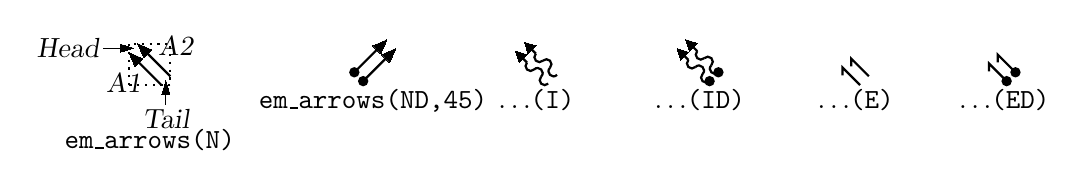
\begin{tikzpicture}[scale=2.54]
% dpic version 2020.03.01 option -g for TikZ and PGF 1.01
\ifx\dpiclw\undefined\newdimen\dpiclw\fi
\global\def\dpicdraw{\draw[line width=\dpiclw]}
\global\def\dpicstop{;}
\dpiclw=0.8bp
\dpiclw=0.8bp
\filldraw[line width=0bp](0.53583,0.053354)
 --(0.465681,0.08422)
 --(0.496546,0.014071) --cycle\dpicstop
\dpicdraw (0.628315,-0.078414)
 --(0.476519,0.073382)\dpicstop
\filldraw[line width=0bp](0.580024,0.097549)
 --(0.509875,0.128414)
 --(0.540741,0.058265) --cycle\dpicstop
\dpicdraw (0.672509,-0.03422)
 --(0.520713,0.117576)\dpicstop
\dpicdraw[dotted](0.465681,-0.078414) rectangle (0.672509,0.128414)\dpicstop
\dpiclw=0.4bp
\filldraw[line width=0bp](0.421111,0.086317)
 --(0.487778,0.106317)
 --(0.421111,0.126317) --cycle\dpicstop
\dpicdraw (0.468444,0.106317)
 --(0.337778,0.106317)\dpicstop
\draw (0.337778,0.106317) node[left=-2bp]{\sl Head};
\filldraw[line width=0bp](0.670412,-0.122984)
 --(0.650412,-0.056317)
 --(0.630412,-0.122984) --cycle\dpicstop
\dpicdraw (0.650412,-0.075651)
 --(0.650412,-0.176317)\dpicstop
\draw (0.650412,-0.176317) node[below=-2bp]{\sl Tail};
\draw (0.546998,0.002903) node[below left=-2bp]{\sl A1};
\draw (0.591192,0.047097) node[above right=-2bp]{\sl A2};
\dpiclw=0.8bp
\draw (0.569095,-0.278414) node[below=-2bp]{\tt em\_arrows(N)};
\filldraw[line width=0bp](1.724278,0.078265)
 --(1.755144,0.148414)
 --(1.684995,0.117549) --cycle\dpicstop
\dpicdraw (1.592509,-0.01422)
 --(1.744305,0.137576)\dpicstop
\filldraw[line width=0bp](1.768472,0.034071)
 --(1.799338,0.10422)
 --(1.729189,0.073354) --cycle\dpicstop
\dpicdraw (1.636704,-0.058414)
 --(1.7885,0.093382)\dpicstop
\dpicdraw[fill=black](1.592509,-0.01422) circle (0.007874in)\dpicstop
\dpicdraw[fill=black](1.636704,-0.058414) circle (0.007874in)\dpicstop
\draw (1.685924,-0.078414) node[below=-2bp]{\tt em\_arrows(ND,45)};
\dpicdraw (2.561973,-0.071092)
 ..controls (2.55221,-0.080855) and (2.53638,-0.080855)
 ..(2.526617,-0.071092)
 ..controls (2.516854,-0.061329) and (2.516854,-0.0455)
 ..(2.526617,-0.035737)\dpicstop
\dpicdraw (2.526617,-0.035737)
 ..controls (2.550188,-0.012166) and (2.514832,0.023189)
 ..(2.491262,-0.000381)\dpicstop
\dpicdraw (2.491262,-0.000381)
 ..controls (2.481499,-0.010144) and (2.46567,-0.010144)
 ..(2.455907,-0.000381)
 ..controls (2.446144,0.009382) and (2.446144,0.025211)
 ..(2.455907,0.034974)\dpicstop
\filldraw[line width=0bp](2.456861,0.073304)
 --(2.399338,0.091543)
 --(2.417577,0.03402) --cycle\dpicstop
\dpicdraw (2.455907,0.034974)
 --(2.407872,0.083008)\dpicstop
\dpicdraw (2.606167,-0.026898)
 ..controls (2.582597,-0.050468) and (2.547241,-0.015113)
 ..(2.570812,0.008457)\dpicstop
\dpicdraw (2.570812,0.008457)
 ..controls (2.580575,0.018221) and (2.580575,0.03405)
 ..(2.570812,0.043813)
 ..controls (2.561048,0.053576) and (2.545219,0.053576)
 ..(2.535456,0.043813)\dpicstop
\dpicdraw (2.535456,0.043813)
 ..controls (2.525693,0.03405) and (2.509864,0.03405)
 ..(2.500101,0.043813)
 ..controls (2.490338,0.053576) and (2.490338,0.069405)
 ..(2.500101,0.079168)\dpicstop
\filldraw[line width=0bp](2.501055,0.117498)
 --(2.443532,0.135737)
 --(2.461771,0.078214) --cycle\dpicstop
\dpicdraw (2.500101,0.079168)
 --(2.452066,0.127203)\dpicstop
\draw (2.502753,-0.078414) node[below=-2bp]{\tt $\ldots$(I)};
\dpicdraw (3.368801,-0.058414)
 ..controls (3.359038,-0.068177) and (3.343209,-0.068177)
 ..(3.333446,-0.058414)
 ..controls (3.323683,-0.048651) and (3.323683,-0.032822)
 ..(3.333446,-0.023059)\dpicstop
\dpicdraw (3.333446,-0.023059)
 ..controls (3.357016,0.000511) and (3.321661,0.035867)
 ..(3.298091,0.012296)\dpicstop
\dpicdraw (3.298091,0.012296)
 ..controls (3.288328,0.002533) and (3.272499,0.002533)
 ..(3.262735,0.012296)
 ..controls (3.252972,0.022059) and (3.252972,0.037889)
 ..(3.262735,0.047652)\dpicstop
\filldraw[line width=0bp](3.263689,0.085981)
 --(3.206167,0.10422)
 --(3.224406,0.046698) --cycle\dpicstop
\dpicdraw (3.262735,0.047652)
 --(3.214701,0.095686)\dpicstop
\dpicdraw (3.412996,-0.01422)
 ..controls (3.389425,-0.03779) and (3.35407,-0.002435)
 ..(3.37764,0.021135)\dpicstop
\dpicdraw (3.37764,0.021135)
 ..controls (3.387403,0.030898) and (3.387403,0.046727)
 ..(3.37764,0.05649)
 ..controls (3.367877,0.066254) and (3.352048,0.066254)
 ..(3.342285,0.05649)\dpicstop
\dpicdraw (3.342285,0.05649)
 ..controls (3.332522,0.046727) and (3.316693,0.046727)
 ..(3.30693,0.05649)
 ..controls (3.297167,0.066254) and (3.297167,0.082083)
 ..(3.30693,0.091846)\dpicstop
\filldraw[line width=0bp](3.307884,0.130176)
 --(3.250361,0.148414)
 --(3.2686,0.090892) --cycle\dpicstop
\dpicdraw (3.30693,0.091846)
 --(3.258895,0.13988)\dpicstop
\dpicdraw[fill=black](3.368801,-0.058414) circle (0.007874in)\dpicstop
\dpicdraw[fill=black](3.412996,-0.01422) circle (0.007874in)\dpicstop
\draw (3.319581,-0.078414) node[below=-2bp]{\tt $\ldots$(ID)};
\dpicdraw (4.121384,-0.078414)
 --(4.032996,0.009974)
 --(4.032996,-0.02931)\dpicstop
\dpicdraw (4.165578,-0.03422)
 --(4.07719,0.054168)
 --(4.07719,0.014884)\dpicstop
\draw (4.099287,-0.078414) node[below=-2bp]{\tt $\ldots$(E)};
\dpicdraw (4.853966,-0.058414)
 --(4.765578,0.029974)
 --(4.765578,-0.00931)\dpicstop
\dpicdraw (4.898161,-0.01422)
 --(4.809772,0.074168)
 --(4.809772,0.034884)\dpicstop
\dpicdraw[fill=black](4.853966,-0.058414) circle (0.007874in)\dpicstop
\dpicdraw[fill=black](4.898161,-0.01422) circle (0.007874in)\dpicstop
\draw (4.841869,-0.078414) node[below=-2bp]{\tt $\ldots$(ED)};
\end{tikzpicture}
\vspace*{-0.5\baselineskip}
